\section{Results}\label{sec:results}

\begin{figure}[t]
    \centering
    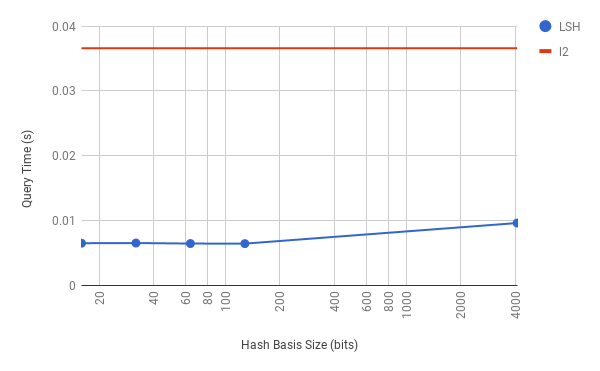
\includegraphics[width=0.5\textwidth]{images/hashing_time_results.png}
    \caption{Hashing query time as a function of basis size. $l_2$ speed plotting in red for comparison. Note that even with 4096 bits, LSH search is significantly faster.}
    \label{fig:speedres}
\end{figure}

We provide an empirical study of our method using two approaches. First we test our primary task of video retrieval. Then, we show how the weights learned by our model provide a good initialization for the action recognition task.

\subsection{Retrieval Results}

\begin{figure}[t]
    \centering
    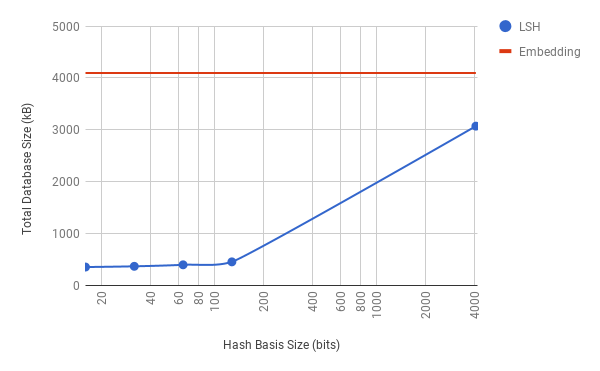
\includegraphics[width=0.5\textwidth]{images/hashing_memory_results.png}
    \caption{Total database size as a function of basis size. Size of the database using the embedding space directly plotted in red for comparison. Again, LSH uses significantly less resources.}
    \label{fig:memres}
\end{figure}

We test several aspects of the video retrieval task. In all tests, we take the UCF101 training set to be our database and select a single probe video from the UCF101 test set. The videos are projected into the 128 dimensional space formed by taking the fc6 output of four six-frame stack of differences distributed uniformly at random through the video. The 128 dimensional representation for each stack of difference is averaged to give the 128 dimensional representation for each video. Our system then returns the top $n$ videos for the given probe image. We tested with $n=5$ but for brevity, only the top match is shown in the qualitative results.

Figure \ref{fig:retres} shows qualitative results of our method. Three representative probe videos were chosen for the figure that had roughly orthogonal motion types. The first video, from the "Cliff Diving" class has fast intricate motions coupled with large camera motions. The second video, from the "Applying Eye Makeup" class, contains constrained small motions. The final video, from the "Writing On Board" class, contains slow and highly controlled motions. We show the top retrieval result using $l_2$ distance in the embedding space and using LSH with basis sizes of 16, 32, 64, 128, and 4096 bits. As shown in the figure, the top retrieval result correctly captures the type of motion in the probe video for $l_2$ distance. Additionally for LSH basis sizes of as small as 64 bits, the motion is still correctly captured. The full retrieval results, along with videos, are provided in the supplementary material.

\begin{figure*}[t]
    \begin{center}
        \begin{tabular}{|c|c|ccccc|}
           \hline
            Probe & $l_2$ & 16 & 32 & 64 & 128 & 4096  \\ \hline \hline
           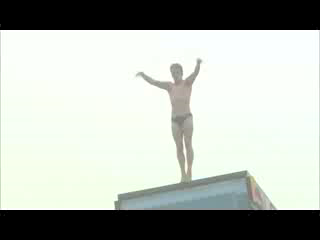
\includegraphics[width=0.1\textwidth]{images/ret_results/diving/probe.png} & 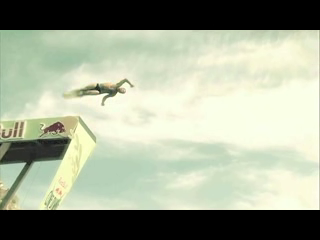
\includegraphics[width=0.1\textwidth]{images/ret_results/diving/l2.png} & 
           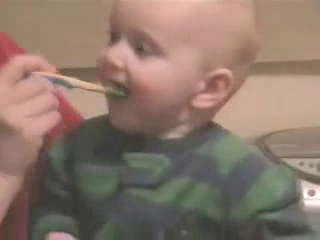
\includegraphics[width=0.1\textwidth]{images/ret_results/diving/16.png} & 
           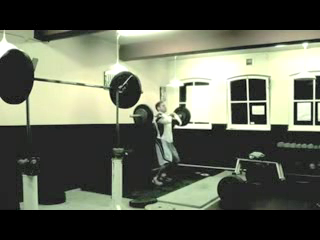
\includegraphics[width=0.1\textwidth]{images/ret_results/diving/32.png} & 
           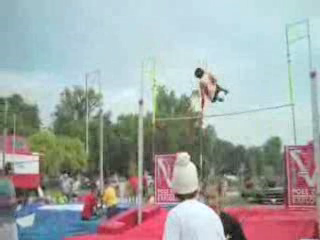
\includegraphics[width=0.1\textwidth]{images/ret_results/diving/64.png} & 
           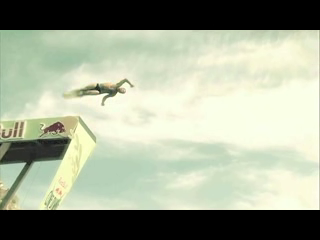
\includegraphics[width=0.1\textwidth]{images/ret_results/diving/128.png} & 
           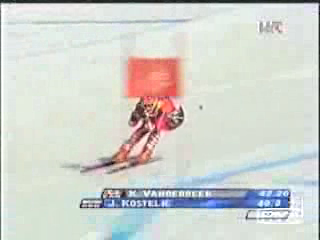
\includegraphics[width=0.1\textwidth]{images/ret_results/diving/4096.png} \\
          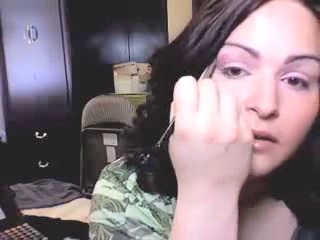
\includegraphics[width=0.1\textwidth]{images/ret_results/eyemakeup/probe.png} & 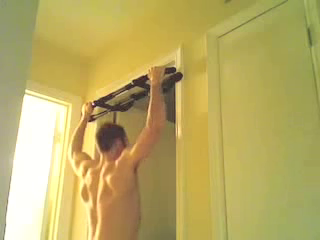
\includegraphics[width=0.1\textwidth]{images/ret_results/eyemakeup/l2.png} &  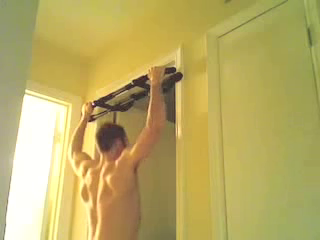
\includegraphics[width=0.1\textwidth]{images/ret_results/eyemakeup/16.png} & 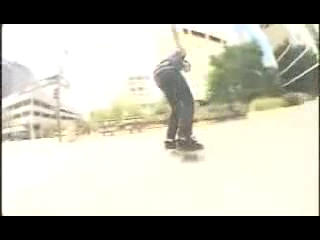
\includegraphics[width=0.1\textwidth]{images/ret_results/eyemakeup/32.png} & 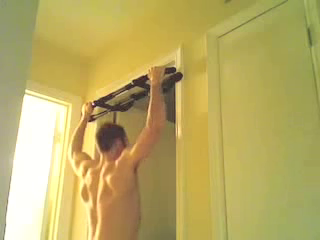
\includegraphics[width=0.1\textwidth]{images/ret_results/eyemakeup/64.png} & 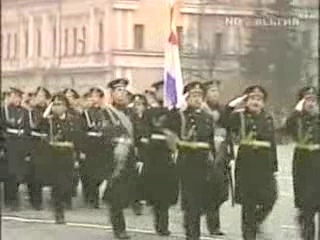
\includegraphics[width=0.1\textwidth]{images/ret_results/eyemakeup/128.png} & 
          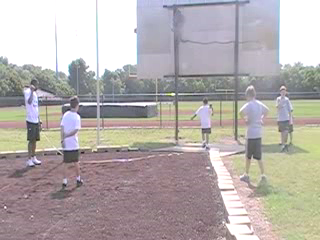
\includegraphics[width=0.1\textwidth]{images/ret_results/eyemakeup/4096.png} \\
          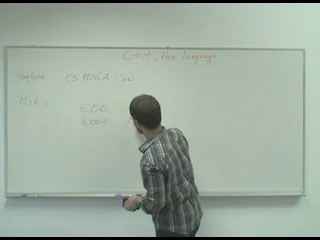
\includegraphics[width=0.1\textwidth]{images/ret_results/writing/probe.png} & 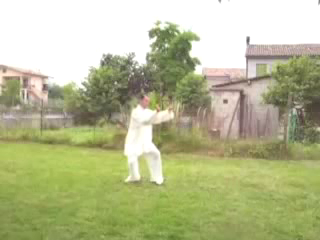
\includegraphics[width=0.1\textwidth]{images/ret_results/writing/l2.png} &  
          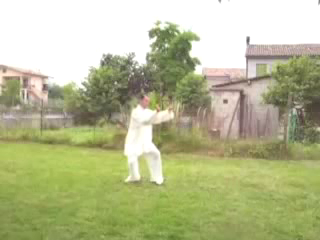
\includegraphics[width=0.1\textwidth]{images/ret_results/writing/16.png} & 
          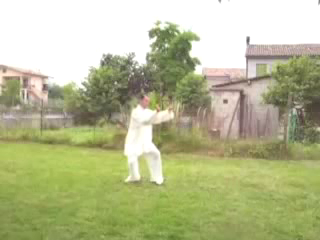
\includegraphics[width=0.1\textwidth]{images/ret_results/writing/32.png} & 
          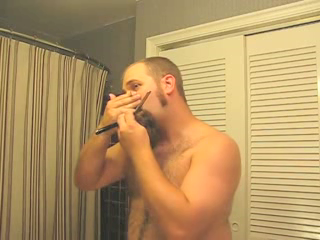
\includegraphics[width=0.1\textwidth]{images/ret_results/writing/64.png} & 
          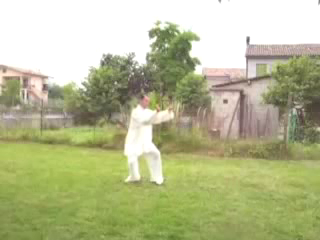
\includegraphics[width=0.1\textwidth]{images/ret_results/writing/128.png} & 
          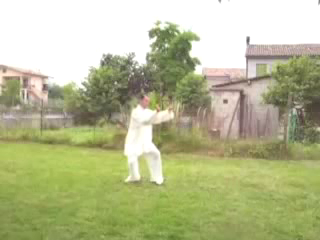
\includegraphics[width=0.1\textwidth]{images/ret_results/writing/4096.png} \\ \hline            
        \end{tabular}
        \caption{Qualitative retrieval results. The learned representations successfully capture similar motions in the videos.}
        \label{fig:retres}
    \end{center}
\end{figure*}

Next we show the quantitative effect of LSH on the system speed and memory usage in Figures \ref{fig:speedres} and \ref{fig:memres}. For these results, the same set of LSH bases, 16, 32, 64, 128, and 4096, are used. The time to retrieve the top $n=5$ videos is computed and the total storage size of the database is reported. As the results show, LSH even with a basis size of 4096 has a significant impact on the speed of retrieval and on the size of the database. Cross referencing with Figure \ref{fig:retres}, this cost efficiency comes with minimal cost in the accuracy of the retrieval results. Even at a basis size of 4096 bits, the LSH database takes up approximately one third less memory than the original database and executes queries approximately four times as quickly.

\subsection{Classification Accuracy Results}

We also conduct a short quantitative study by using our weights as the initialization for AlexNet action recognition and fine-tuning the network. We follow the fine-tuning procedure in \cite{fernando2017self} for both the original O3N network and for our dual-loss architecture. The results are shown in \ref{fig:classres}, our networks weights give an improvement of \todo\% over O3N initialization.

We briefly review the fine-tuning procedure. We start with the standard AlexNet network. The convolutional layers are initialized with our weights, the fully connected layers, which now have 4096 activations, are initialized with random weights. The network is then trained for the action recognition task by using a $10^{-4}$ learning rate for the convolutional layers , which should already have reasonable weights according to our hypothesis. The fully-connected layers are trained with a $10^{-2}$ learning rate since they start with random weights. 

We tested several different initialization to ensure a good comparison. For a baseline, we start from random weights and train with the $10^{-2}$ learning rate for all layers. For O3N and ours, we follow the fine tuning procedure described above. We also follow the fine-tuning procedure starting from ImageNet weights. This gives the best performance but it is worth noting that our method is only \todo\% worse while requiring no supervision.

\begin{table}
    \centering
    \begin{tabu} to 0.5\textwidth {|X[l]|X[c]|}
        \hline
        Initialization & Accuracy (\%) \\ \hline \hline
        Random & \todo \\ \hline
        ImageNet & \textbf{70.8} \\ \hline
        O3N Initialization & 65.3 \\ \hline
        Ours & \todo \\ \hline
    \end{tabu}
    \caption{Fine-tuned classification accuracy for different weight initializations.}
    \label{fig:classres}
\end{table}



